\documentclass[letterpaper,10pt]{article}

%\setlength{\parindent}{0in}
%\usepackage{fullpage} 
\usepackage{amsmath}
\usepackage{amssymb}
\usepackage{enumerate}
\usepackage{graphicx}
\usepackage{dcolumn}
\oddsidemargin 0.0in
\textwidth 6.5in
\newcolumntype{.}{D{.}{.}{-1}}

%opening
\title{Homework 1}
\author{Steve Mazza}
\date{October 18, 2011}

\begin{document}
\maketitle

\begin{enumerate}
\item
\begin{enumerate}
\item\ \\
\begin{center}
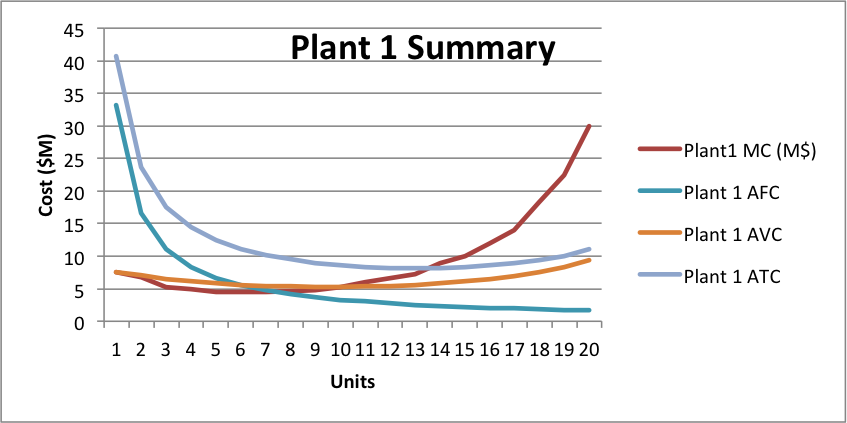
\includegraphics[scale=0.75]{Plant1Plot.png} \\
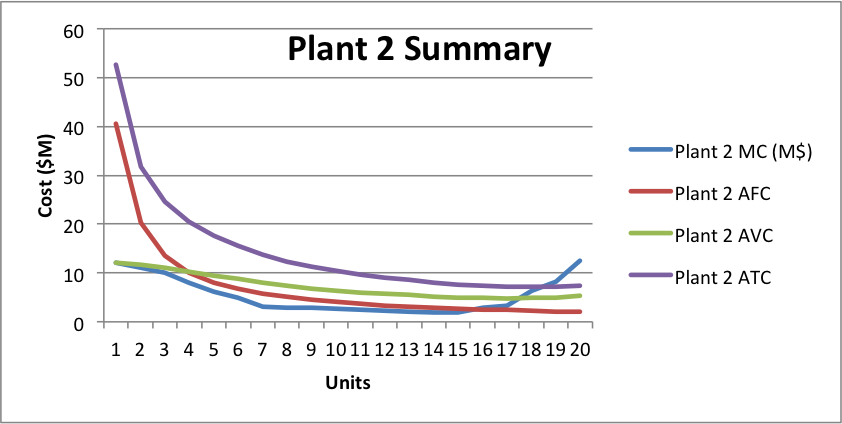
\includegraphics[scale=0.75]{Plant2Plot.png}
\end{center}
\item Prefer Plant 1 for 5 units and Plant 2 for 20 units.
\end{enumerate}

\item There are several sources of both fixed and variable costs for producing drone aircraft.  Obvious sources of fixed costs include amortization of facility, equipment, appurtenances, machinery, and previously held leases (not directly associated with production).  Some classes of employee expenses are also considered fixed costs, for example most \emph{exempt} or salaried employees especially those associated with middle and upper management roles.  Miscellaneous fixed cost items also include insurance, most benefits, and a portion of utilities.  Non-obvious fixed costs may include amortization of research and development, employee education and training, and facility maintenance.
\par Obvious sources of variable costs include hourly labor, supplies and materials, shipping, and a portion of the utilities.  Insurance, benefits, and employee training will also increase commensurate with an increase in the work force.

\item Using the second fundamental proposition of marginal reasoning we determine that \[\frac{\mbox{Mobile Teams}}{80000}=\frac{\mbox{TV Commercials}}{60000}=\frac{\mbox{Newspaper Ads}}{40000}=0.0006\]This value is achieved for three (3) units for Mobile Teams, there (3) units for TV Commercials, and five (5) units for Newspaper Ads.  See accompanying Excel spreadsheet for supporting documentation.
\begin{table}[htdp]
\begin{center}
\begin{tabular}{lrrr}
\hline
Type & Cost & Quantity & Extension \\
\hline
Mobile Teams & 80000 & 3 & 240000 \\
TV Commercials & 60000 & 3 & 180000 \\
Newspaper Ads & 40000 & 5 & 200000 \\
\hline
& & Total & 620000
\end{tabular}
\end{center}
\label{default}
\end{table}

\item A cost estimating relationship (CER) is a mechanism by which one studies a process to determine a reasonable model for arriving at cost as a function of objective, quantifiable, independent variables.  A CER is a model for cost estimation and, inasmuch, is not precise.  The most frequently employed mechanism for arriving at a reasonable model is to use regression analysis, a method of curve-fitting known data points to estimate an unknown value (e.g., cost).
\par The general prescription for arriving at a cost estimating relationship is a series of evaluate-test iterations that often begins with data collection.  Once data is collected it is analyzed to determine predominant relationships.  These relationships are tested against the data and more is collected if necessary (or possible).  Only after arriving at a confidence in both the data and relationships do we try to fit a regression model.  Assuming we can rely on the data, the biggest challenge is to properly identify the independent variables.
\par Important to note is that CER's are imprecise.  They are based largely on what we can infer from historical data and, even with the largest data sets, are non-deterministic.  The formula for regression always carries the term $\varepsilon$ for error which is an important statistical measure for the CER.  Error is influenced by the choice of independent variables, is reflected in the fit of the regression curve, and is indicative of our overall confidence in the estimate.
\par Using least squares regression allows us to fit an equation for a line\[y_{i}=b_{0}+b_{1}x_{i}+e_{i}\]such that it passes through a data set as centrally as possible.  This is accomplished by choosing $b_{0}$ and $b_{1}$ that minimizes the sum of their residuals squared.  We assess the quality of our model by inspecting standard error, coefficient of variation, coefficient of determination, the $t$-statistic, the $f$-statistic, and analysis of variance.
\par Diagnosis of errors in the CER involves inspecting the plot residuals.  There should be no noticeable pattern.  If there is, you likely missed something in your model.
\end {enumerate}
\end{document}